\chapter{Random Forests}\label{ch:forest}

\begin{remark}{Outline}
In this chapter, we present the well-known family of \textit{Random Forests}
methods. In Section~\ref{sec:4:bias-variance}, we first describe the
bias-variance decomposition of the prediction error and then present, in
Section~\ref{sec:4:ensemble}, how aggregating randomized models through
ensembles reduces the prediction error by decreasing the variance term in this
decomposition. In Section~\ref{sec:4:random-forests}, we revisit Random Forests ant its variants and
study how randomness introduced into the decision tree induction algorithm can
reduce prediction error by decorrelating the decision trees in the ensemble.
Finally, the consistency of forests of randomized trees is explored in
Section~\ref{sec:4:consistency}.
\end{remark}


\section{Bias-variance decomposition}
\label{sec:4:bias-variance}

In section~\ref{sec:2:performance-evaluation}, we defined the generalization
error of a model $\varphi_{\cal L}$ as its expected prediction error
according to some loss function $L$
\begin{equation}
Err(\varphi_{\cal L}) = \mathbb{E}_{X,Y} \{ L(Y, \varphi_{\cal L}(X)) \}.
\end{equation}
Similarly, the expected prediction error of $\varphi_{\cal L}$ at $X=\mathbf{x}$
can be expressed as
\begin{equation}
Err(\varphi_{\cal L}(\mathbf{x})) = \mathbb{E}_{Y|X=\mathbf{x}} \{ L(Y, \varphi_{\cal L}(\mathbf{x})) \}.\label{eqn:4:generalization-error:x}
\end{equation}

In regression, this latter form of the expected prediction error additively
decomposes into bias and variance terms which together constitute a very useful
framework for diagnosing the prediction error of a model. In classification, a
similar decomposition is more difficult to obtain. Yet, the
concepts of bias and variance can be transposed in several ways to
classification, thereby providing comparable frameworks for studying the
prediction error of classifiers.


\subsection{Regression}
\label{sec:bias-variance:regression}

In regression, assuming that $L$ is the squared error loss, the expected
prediction error of a model $\varphi_{\cal L}$ at a given point $X=\mathbf{x}$
can be rewritten with respect to the Bayes model $\varphi_B$:
\begin{align}
& Err(\varphi_{\cal L}(\mathbf{x})) \nonumber \\
&= \mathbb{E}_{Y|X=\mathbf{x}} \{ (Y - \varphi_{\cal L}(\mathbf{x}))^2 \} \nonumber \\
&= \mathbb{E}_{Y|X=\mathbf{x}} \{ (Y -\varphi_B(\mathbf{x}) + \varphi_B(\mathbf{x}) - \varphi_{\cal L}(\mathbf{x}))^2 \} \nonumber \\
&= \mathbb{E}_{Y|X=\mathbf{x}} \{ (Y -\varphi_B(\mathbf{x}))^2  \} + \mathbb{E}_{Y|X=\mathbf{x}} \{ (\varphi_B(\mathbf{x}) - \varphi_{\cal L}(\mathbf{x}))^2 \} \nonumber \\
& \quad+ \mathbb{E}_{Y|X=\mathbf{x}} \{ 2 (Y - \varphi_B(\mathbf{x}))(\varphi_B(\mathbf{x}) - \varphi_{\cal L}(\mathbf{x})) \} \nonumber \\
&= \mathbb{E}_{Y|X=\mathbf{x}} \{ (Y -\varphi_B(\mathbf{x}))^2 \} + \mathbb{E}_{Y|X=\mathbf{x}} \{ (\varphi_B(\mathbf{x}) - \varphi_{\cal L}(\mathbf{x}))^2 \} \nonumber \\
&= Err(\varphi_B(\mathbf{x})) +  (\varphi_B(\mathbf{x}) - \varphi_{\cal L}(\mathbf{x}))^2 \label{eqn:4:decomp1}
\end{align}
since $\mathbb{E}_{Y|X=\mathbf{x}} \{ Y - \varphi_B(\mathbf{x}) \} =
\mathbb{E}_{Y|X=\mathbf{x}} \{ Y \} - \varphi_B(\mathbf{x}) = 0$ by definition
of the Bayes model in regression. In this form, the first term in the last
expression of Equation~\ref{eqn:4:decomp1} corresponds to the (irreducible)
residual error  at $X=\mathbf{x}$ while the second term represents the
discrepancy of $\varphi_{\cal L}$ from the Bayes model. The further from the
Bayes model, the more sub-optimal the model and the larger the error.

If we further assume that the learning set ${\cal L}$ is itself a random
variable (sampled from the population $\Omega$) and that the learning algorithm is deterministic, then the expected
discrepancy with the Bayes model can further be re-expressed in terms of the
average prediction $\mathbb{E}_{\cal L} \{ \varphi_{\cal L}(\mathbf{x}) \}$
over the models learned from all possible learning sets of size $N$:
\begin{align}
& \mathbb{E}_{\cal L} \{ (\varphi_B(\mathbf{x}) - \varphi_{\cal L}(\mathbf{x}))^2 \}\nonumber \\
&= \mathbb{E}_{\cal L} \{ (\varphi_B(\mathbf{x}) - \mathbb{E}_{\cal L} \{ \varphi_{\cal L}(\mathbf{x}) \} + \mathbb{E}_{\cal L} \{ \varphi_{\cal L}(\mathbf{x}) \} - \varphi_{\cal L}(\mathbf{x}))^2 \} \nonumber \\
&= \mathbb{E}_{\cal L} \{ (\varphi_B(\mathbf{x}) - \mathbb{E}_{\cal L} \{ \varphi_{\cal L}(\mathbf{x}) \} )^2 \} + \mathbb{E}_{\cal L} \{ (\mathbb{E}_{\cal L} \{ \varphi_{\cal L}(\mathbf{x}) \} - \varphi_{\cal L}(\mathbf{x}))^2 \} \}\nonumber \\
& \quad+ \mathbb{E}_{\cal L} \{ 2(\varphi_B(\mathbf{x}) - \mathbb{E}_{\cal L} \{ \varphi_{\cal L}(\mathbf{x}) \})(\mathbb{E}_{\cal L} \{ \varphi_{\cal L}(\mathbf{x}) \} - \varphi_{\cal L}(\mathbf{x}))\} \nonumber \\
&= \mathbb{E}_{\cal L} \{ (\varphi_B(\mathbf{x}) - \mathbb{E}_{\cal L} \{ \varphi_{\cal L}(\mathbf{x}) \} )^2 \} + \mathbb{E}_{\cal L} \{ (\mathbb{E}_{\cal L} \{ \varphi_{\cal L}(\mathbf{x}) \} - \varphi_{\cal L}(\mathbf{x}))^2 \} \}\nonumber \\
&= (\varphi_B(\mathbf{x}) - \mathbb{E}_{\cal L} \{ \varphi_{\cal L}(\mathbf{x}) \} )^2 + \mathbb{E}_{\cal L} \{ (\mathbb{E}_{\cal L} \{ \varphi_{\cal L}(\mathbf{x}) \} - \varphi_{\cal L}(\mathbf{x}))^2 \}
\end{align}
since $\mathbb{E}_{\cal L}\{ \mathbb{E}_{\cal L} \{ \varphi_{\cal
L}(\mathbf{x}) \} - \varphi_{\cal L}(\mathbf{x}) \} =  \mathbb{E}_{\cal L} \{
\varphi_{\cal L}(\mathbf{x}) \} -  \mathbb{E}_{\cal L} \{ \varphi_{\cal
L}(\mathbf{x}) \} = 0$. In summary, the expected generalization error additively
decomposes as formulated in Theorem~\ref{thm:bias-variance}.

\begin{theorem}\label{thm:bias-variance}
For the square error loss, the bias-variance decomposition of the expected
generalization error $\mathbb{E}_{\cal L} \{ Err(\varphi_{\cal L}(\mathbf{x}))
\}$ at $X=\mathbf{x}$ is
\begin{equation}
\mathbb{E}_{\cal L} \{ Err(\varphi_{\cal L}(\mathbf{x})) \} = \text{noise}(\mathbf{x}) + \text{bias}^2(\mathbf{x}) + \text{var}(\mathbf{x}),
\end{equation}
where
\begin{align*}
\text{noise}(\mathbf{x}) &= Err(\varphi_B(\mathbf{x})), \\
\text{bias}^2(\mathbf{x}) &= (\varphi_B(\mathbf{x}) - \mathbb{E}_{\cal L} \{ \varphi_{\cal L}(\mathbf{x}) \} )^2, \\
\text{var}(\mathbf{x}) &= \mathbb{E}_{\cal L} \{ (\mathbb{E}_{\cal L} \{ \varphi_{\cal L}(\mathbf{x}) \} - \varphi_{\cal L}(\mathbf{x}))^2 \}.
\end{align*}
\end{theorem}

This bias-variance decomposition of the generalization error is due to
\citet{geman:1992} and was first proposed in the context of neural networks.
The first term, $\text{noise}(\mathbf{x})$, is the residual error. It is
entirely independent of both the learning algorithm and the learning set and
provides for any model a theoretical lower bound on its generalization error.
The second term, $\text{bias}^2(\mathbf{x})$, measures the discrepancy between
the average prediction and the prediction of the Bayes model. Finally, the
third term, $\text{var}(\mathbf{x})$, measures the variability of the
predictions at $X=\mathbf{x}$ over the models learned from all possible
learning sets. All three terms are illustrated in Figure~\ref{fig:bias-variance}
for a toy regression problem. Both $\text{noise}(\mathbf{x})$ and
$\text{var}(\mathbf{x})$ measures the spread of the two densities while
$\text{bias}^2(\mathbf{x})$ is the distance between their means.

\begin{figure}
    \centering
    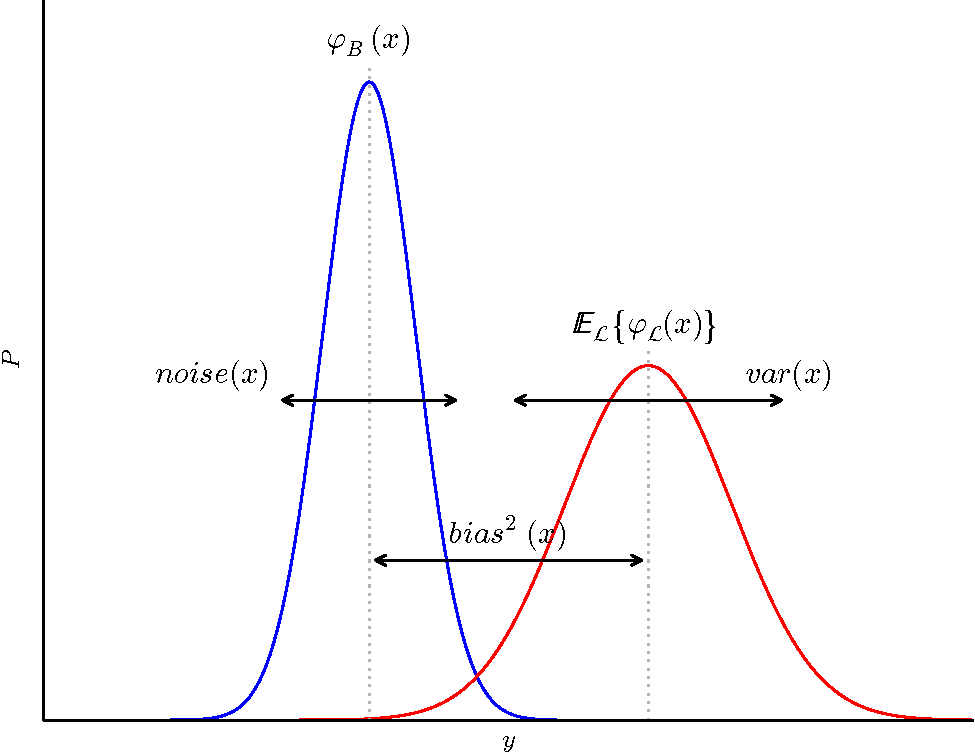
\includegraphics[width=0.9\textwidth]{figures/ch4_bias_variance.pdf}
    \caption{Residual error, bias and variance at $X=\mathbf{x}$. (Figure inspired from \citep{geurts:2002}.)}
    \label{fig:bias-variance}
\end{figure}

As a typical example, the bias-variance decomposition framework can be used as
a tool for diagnosing underfitting and overfitting (as previously introduced in
Section \ref{sec:2:model-selection}). The upper plots in
Figure~\ref{fig:overfitting} illustrate in light red predictions $\varphi_{\cal
L}(\mathbf{x})$ for polynomials of degree $1$, $5$ and $15$ learned over random
learning sets ${\cal L}$ sampled from a noisy cosinus function. Predictions
$\mathbb{E}_{\cal L} \{ \varphi_{\cal L}(\mathbf{x}) \}$ of the average model
are represented by the thick red lines. Predictions for the model learned over
the learning set represented by the blue dots are represented in gray.
Predictions of the Bayes model are shown in blue and coincide with the unnoised
cosinus function that defines the regression problem. The lower plots in the
figure illustrate the bias-variance decomposition of the expected
generalization error of the polynomials.

\begin{figure}
    \hspace{-0.75cm}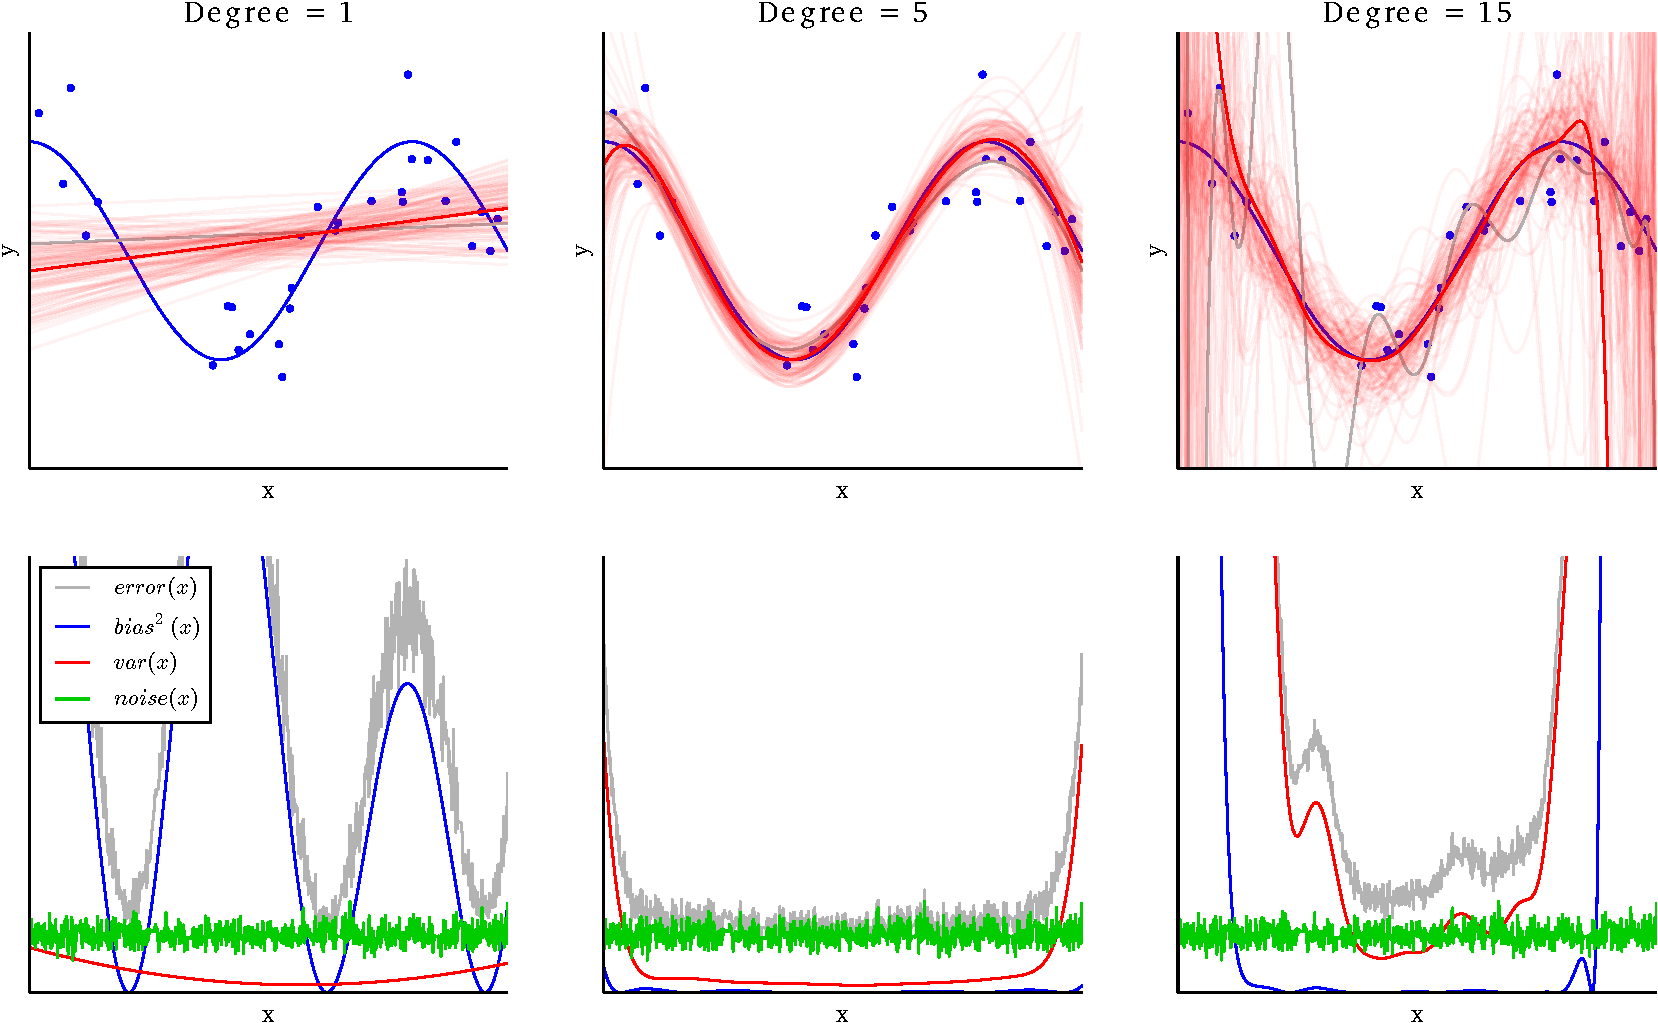
\includegraphics[width=1.1\textwidth]{figures/ch4_overfitting.pdf}
    \caption{Bias-variance decomposition of the expected generalization error for polynomials of degree $1$, $5$ and $15$.}
    \label{fig:overfitting}
\end{figure}

Clearly, polynomials of degree $1$ (left) suffer from underfitting. In terms of
bias and variance, this translates into low variance but high bias as shown in
the lower left plot of Figure~\ref{fig:overfitting}. Indeed, due to the low
degree of the polynomials (i.e., due to the low model complexity), the
resulting models are almost all identical and  the variability of the
predictions from one model to another is therefore quite low. Also, because of
low complexity, none of them really fits the trend of the training points, even
approximately, which implies that the average model is far from approximating
the Bayes model. This results in high bias. On the other hand, polynomials of
degree $15$ (right) suffer from overfitting. In terms of bias and variance, the
situation is the opposite. Predictions have low bias but high variance, as
shown in the lower right plot of Figure~\ref{fig:overfitting}. The variability
of the predictions is large because the high degree of the polynomials (i.e.,
the high model complexity) captures noise in the learning set. Indeed, compare
the gray line with the blue dots -- they almost all intersect. Put otherwise,
small changes in the learning set result in large changes in the obtained model
and therefore in its predictions. By contrast, the average model is now quite
close from the Bayes model, which results in low bias\footnote{Note however the
Gibbs-like phenomenon resulting in both high variance and high bias at the
boundaries of ${\cal X}$.}. Finally, polynomials of degree $5$ (middle) are
neither too simple nor too complex. In terms of bias and variance, the trade-
off is well-balanced between the two extreme situations. Bias and variance are
neither too low nor too large.


\subsection{Classification}
\label{sec:bias-variance:classification}

In direct analogy with the bias-variance decomposition for the square error
loss, similar decompositions have been proposed in the literature for the
expected generalization error based on the zero-one loss, i.e., for
$\mathbb{E}_{\cal L}\{ \mathbb{E}_{Y|X=\mathbf{x}} \{ 1(\varphi_{\cal L}(x)
\neq Y) \} \} = P_{{\cal L},Y|X=\mathbf{x}}(\varphi_{\cal L}(\mathbf{x}) \neq
Y)$. Most notably, \citet{dietterich:1995}, \citet{breiman:1996},
\citet{kohavi:1996} and \citet{tibshirani:1996} have all developed additive
decompositions similar to Theorem~\ref{thm:bias-variance} by redefining the
concepts of bias and variance in the case of classification. While these
efforts have all provided useful insight into the nature of classification
error, none of them really have provided a seductively as simple and
satisfactory framework as in regression (for reviews, see
\citep{friedman:1997,geurts:2002,james:2003}).

An interesting connection with Theorem~\ref{thm:bias-variance} however is to
remark that classification algorithms usually work by computing estimates
\begin{equation}
p_{\cal L}(Y=c|X=\mathbf{x})
\end{equation}
of the conditional class probability (e.g.,
$p_{\cal L}(Y=c|X=\mathbf{x}) = p(c|t)$ in decision trees, where $t$ is the
leaf reached by $\mathbf{x}$) and then deriving a classification rule by
predicting the class that maximizes this estimate, that is:
\begin{equation}\label{eqn:4:classificaton-rule}
\varphi_{\cal L}(\mathbf{x}) = \argmax_{c \in {\cal Y}} p_{\cal L}(Y=c|X=\mathbf{x})
\end{equation}
As such, a direction for studying classification models is the relate the
bias-variance decomposition of these numerical estimates to the expected
misclassification error of classification rule~\ref{eqn:4:classificaton-rule}.

We now reproduce the results of \citet{friedman:1997} who made this connection
explicit for the case of binary classification. Let us first decompose the
expected classification error into an irreducible part associated with the
random nature of the output $Y$ and a reducible part that depends on
$\varphi_{\cal L}(\mathbf{x})$, in analogy with Equation~\ref{eqn:4:decomp1}
for the square error loss. (Note that, to simplify notations, we assume that
all probabilities based on the random variable $Y$ is with respect to the
distribution of $Y$ at $X=\mathbf{x}$.)
\begin{align}
& \mathbb{E}_{\cal L}\{ \mathbb{E}_{Y|X=\mathbf{x}} \{ 1(\varphi_{\cal L}(x) \neq Y) \} \}  \\
&= P_{{\cal L}}(\varphi_{\cal L}(\mathbf{x}) \neq Y) \nonumber \\
&= \begin{aligned}[t]
    1 &- P_{\cal L}(\varphi_{\cal L}(\mathbf{x}) = \varphi_B(\mathbf{x})) P(\varphi_B(\mathbf{x})=Y) \nonumber \\
      &- P_{\cal L}(\varphi_{\cal L}(\mathbf{x}) \neq \varphi_B(\mathbf{x})) P(\varphi_B(\mathbf{x})\neq Y) \nonumber
   \end{aligned}\nonumber \\
&= \begin{aligned}[t]
    &P(\varphi_B(\mathbf{x})\neq Y) + P_{\cal L}(\varphi_{\cal L}(\mathbf{x})\neq \varphi_B(\mathbf{x})) \nonumber \\
    &- 2 P_{\cal L}(\varphi_{\cal L}(\mathbf{x})\neq \varphi_B(\mathbf{x})) P(\varphi_B(\mathbf{x})\neq Y)  \nonumber \\
   \end{aligned}\nonumber \\
&= P(\varphi_B(\mathbf{x})\neq Y) + P_{\cal L}(\varphi_{\cal L}(\mathbf{x})\neq \varphi_B(\mathbf{x}))(2 P(\varphi_B(\mathbf{x}) = Y) - 1) \nonumber
\end{align}

In this form, the first term is the irreducible error of the Bayes model. The
second term is the increased error due to the misestimation of the optimal
decision boundary. The probability $P_{\cal L}(\varphi_{\cal L}(\mathbf{x})\neq
\varphi_B(\mathbf{x}))$  is the probability for the model of making a decision
which is different from the decision of the Bayes model. This happens
when the estimate $p_{\cal L}(Y=\varphi_B(\mathbf{x}))$ is lower
than $0.5$, that is:
\begin{equation}\label{eqn:4:prob-diff-from-bayes}
P_{\cal L}(\varphi_{\cal L}(\mathbf{x})\neq \varphi_B(\mathbf{x})) = P_{\cal L}(p_{\cal L}(Y=\varphi_B(\mathbf{x})) < 0.5)
\end{equation}
As Figure~\ref{fig:estimate-distribution} illustrates, probability~\ref{eqn:4:prob-diff-from-bayes}
in fact corresponds to the tail area on the left side
of the decision threshold (at 0.5) of the distribution of the estimate.

\begin{figure}
    \centering
    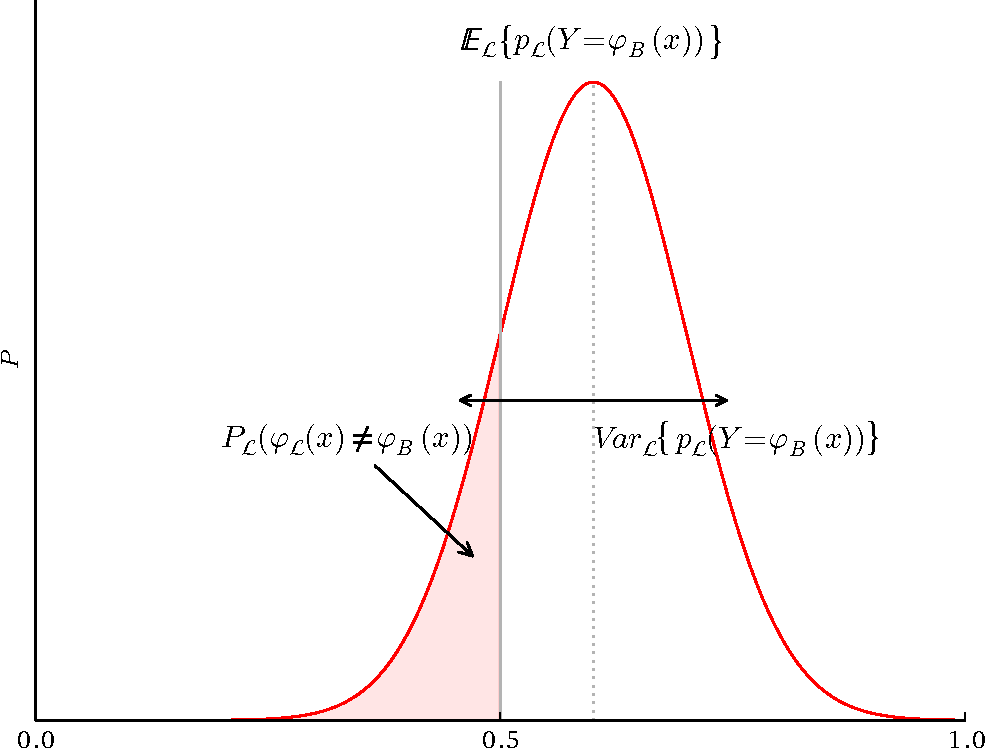
\includegraphics[width=0.9\textwidth]{figures/ch4_estimate_distribution.pdf}
    \caption{Probability distribution of $p_{\cal L}(Y=\varphi_B(\mathbf{x}))$.}
    \label{fig:estimate-distribution}
\end{figure}

If we now further assume\footnote{For single decision trees, the normal
assumption is certainly not satisfied in all cases, but the qualitative
conclusions are still generally valid. When the computations of the estimates
involve some averaging process, e.g., as further developed in the case of
ensemble of randomized trees, this approximation is however fairly reasonable.}
that the estimate $p_{\cal L}(Y=\varphi_B(\mathbf{x}))$ is normally distributed,
then probability~\ref{eqn:4:prob-diff-from-bayes} can be computed explicitly
from its mean and variance:
\begin{equation}
P_{\cal L}(p_{\cal L}(Y=\varphi_B(\mathbf{x})) < 0.5) = \Phi(\frac{0.5 - \mathbb{E}_{\cal L}\{ p_{\cal L}(Y=\varphi_B(\mathbf{x})) \}}{\sqrt{\text{Var}_{\cal L}\{ p_{\cal L}(Y=\varphi_B(\mathbf{x})) \}}})
\end{equation}
where $\Phi(x)=\frac{1}{\sqrt{2\pi}} \int_{-\infty}^x \exp(-\frac{t^2}{2}) dt$
is the cumulative distribution function of the standard normal distribution.
In summary, the expected generalization error additively
decomposes as formulated in Theorem~\ref{thm:bias-variance:classification}.

\begin{theorem}\label{thm:bias-variance:classification}
For the zero-one loss and binary classification, the expected
generalization error $\mathbb{E}_{\cal L} \{ Err(\varphi_{\cal L}(\mathbf{x}))
\}$ at $X=\mathbf{x}$ decomposes as follows:

\begin{align}
\mathbb{E}_{\cal L} \{ Err(\varphi_{\cal L}(\mathbf{x})) \} &= P(\varphi_B(\mathbf{x})\neq Y) \\
                                                            &+ \Phi(\frac{0.5 - \mathbb{E}_{\cal L}\{ p_{\cal L}(Y=\varphi_B(\mathbf{x})) \}}{\sqrt{\text{Var}_{\cal L}\{ p_{\cal L}(Y=\varphi_B(\mathbf{x})) \}}}) (2 P(\varphi_B(\mathbf{x}) = Y) - 1) \nonumber
\end{align}
\end{theorem}

As a result, Theorem~\ref{thm:bias-variance:classification} establishes a
direct connection between the regression variance of the estimates and the
classification error of the resulting model. In practice, this decomposition
has important consequences:
\begin{itemize}
\item When the expected probability estimate $\mathbb{E}_{\cal L}\{ p_{\cal L}(Y=\varphi_B(\mathbf{x}) \}$
      for the true majority class is greater than $0.5$, a reduction of
      variance of the estimate results in a decrease of the total misclassification
      error. If $\text{Var}_{\cal L}\{ p_{\cal L}(Y=\varphi_B(\mathbf{x})) \} \to 0$,
      then $\Phi \to 0$ and the expected generalization error tends to the error of the Bayes model.
      In particular, the generalization error can be driven to its minimum
      value whatever the regression bias of the estimate (at least as long as $\mathbb{E}_{\cal L}\{ p_{\cal L}(Y=\varphi_B(\mathbf{x}) \} > 0.5$).
\item Conversely, when $\mathbb{E}_{\cal L}\{ p_{\cal L}(Y=\varphi_B(\mathbf{x}) \} < 0.5$,
      a decrease of variance might actually increase the total misclassification error.
      If $\text{Var}_{\cal L}\{ p_{\cal L}(Y=\varphi_B(\mathbf{x})) \} \to 0$,
      then $\Phi \to 1$ and the error is maximal.
\end{itemize}


\section{Ensemble methods}
\label{sec:4:ensemble}

Both theorems~\ref{thm:bias-variance} and \ref{thm:bias-variance:classification}
reveal the role of variance in the expected generalization error of a model. In
light of these results, a sensible approach for reducing generalization error
would therefore consist in driving down the prediction variance, provided the
respective bias can be kept the same or not be increased too much.

As it happens, \textit{ensemble methods} constitute a beautifully simple way to
do just that. Specifically, the core principle of ensemble methods is to
introduce random perturbations into the learning procedure in order to produce
several different models from a single learning set ${\cal L}$ and then to
combine the predictions of those models to form the prediction of the ensemble.
How predictions are combined and why does it help is formally studied in the
next sections.


\subsection{Randomized models}

Given a learning set ${\cal L}$, a learning algorithm ${\cal A}$
deterministically produces a model ${\cal A}(\theta, {\cal L})$, denoted
$\varphi_{{\cal L},\theta}$, where $\theta$ are hyper-parameters controlling
the execution of ${\cal A}$. Let us assume that $\theta$ includes a random seed
parameter for mimicking some stochastic behavior in ${\cal A}$, hence producing
(pseudo-)randomized models that are more or less different from one random seed
to another. (We defer the discussion on specific random perturbations in the
case of decision trees to Section~\ref{sec:4:random-forests}.)

In this context, the bias-variance decomposition can be extended to account for
everything that is random, hence considering both ${\cal L}$ and $\theta$ as
random variables\footnote{From now on, and without loss of generality, we
assume that the random variable $\theta$ only controls the randomness of the
learning algorithm.}.
Accordingly, theorems~\ref{thm:bias-variance} and \ref{thm:bias-variance:classification}
naturally extend to the expected generalization error
$\mathbb{E}_{{\cal L},\theta} \{ Err(\varphi_{{\cal L},\theta}(\mathbf{x})) \}$
of the randomized model $\varphi_{{\cal L},\theta}$ by replacing expectations
$\mathbb{E}_{\cal L} \{ . \}$ and variances $\text{Var}_{\cal L} \{ . \}$ with
their respective counterparts $\mathbb{E}_{{\cal L},\theta} \{ . \}$ and
$\text{Var}_{{\cal L},\theta} \{ . \}$ computed over the joint distribution of
${\cal L}$ and $\theta$. In regression, the bias-variance decomposition
of the square error loss thus becomes:
\begin{equation}
\mathbb{E}_{{\cal L},\theta} \{ Err(\varphi_{{\cal L},\theta}(\mathbf{x})) \} = \text{noise}(\mathbf{x}) + \text{bias}^2(\mathbf{x}) + \text{var}(\mathbf{x}),
\end{equation}
where
\begin{align}
\text{noise}(\mathbf{x}) &= Err(\varphi_B(\mathbf{x})), \\
\text{bias}^2(\mathbf{x}) &= (\varphi_B(\mathbf{x}) - \mathbb{E}_{{\cal L},\theta} \{ \varphi_{{\cal L},\theta}(\mathbf{x}) \} )^2, \\
\text{var}(\mathbf{x}) &= \mathbb{E}_{{\cal L},\theta} \{ (\mathbb{E}_{{\cal L},\theta} \{ \varphi_{{\cal L},\theta}(\mathbf{x}) \} - \varphi_{{\cal L},\theta}(\mathbf{x}))^2 \}.
\end{align}

In this form, variance now accounts for both the prediction variability due to
the randomness of the learning set ${\cal L}$ and the variability due to the
randomness of the learning algorithm itself. As a result, the variance of a
randomized algorithm is usually strictly larger than the variance of its
deterministic counterpart. Depending on the strength of randomization, bias
also usually increases, but often to a smaller extent than variance.


\subsection{Combining randomized models}

Let us assume a set of $M$ randomized models $\{\varphi_{{\cal L}, \theta_m} |
m = 1, \dots, M \}$, all learned on the same data ${\cal L}$ but each built
from an independent random seed $\theta_m$. Ensemble methods work by combining
the predictions of these models into a new \textit{ensemble} model, denoted
$\psi_{{\cal L},\theta_1,\dots,\theta_M}$, such that the expected
generalization error of the ensemble is (hopefully) smaller than the expected
generalization error of the individual randomized models.

In regression, the most common way to combine the randomized models into an
ensemble is to average their predictions to form the final prediction:
\begin{equation}
\psi_{{\cal L},\theta_1,\dots,\theta_M}(\mathbf{x}) = \frac{1}{M} \sum_{m=1}^M \varphi_{{\cal L},\theta_m}(\mathbf{x})
\end{equation}

In classification, predictions are usually aggregated by considering the
models in the ensemble as a committee  and then resorting to majority voting to
form the final prediction:
\begin{equation}
\psi_{{\cal L},\theta_1,\dots,\theta_M}(\mathbf{x}) = \argmax_{c \in {\cal Y}}  \sum_{m=1}^M 1(\varphi_{{\cal L},\theta_m}(\mathbf{x})=c)
\end{equation}
When individual models provide class probability estimates $p_{{\cal L},\theta m}(Y=c|X=\mathbf{x})$,
a natural alternative to majority voting consists in averaging the class probability estimates
and then predict the class which is the most likely:
\begin{equation}\label{eqn:4:avg-estimate}
\psi_{{\cal L},\theta_1,\dots,\theta_M}(\mathbf{x}) = \argmax_{c \in {\cal Y}} \frac{1}{M} \sum_{m=1}^M p_{{\cal L},\theta m}(Y=c|X=\mathbf{x})
\end{equation}
As empirically investigated by \citet{breiman:1996b}, both approaches yield
results that are virtually identical. From a practical point of view however,
Equation~\ref{eqn:4:avg-estimate} has the advantage of providing accurate class
probability estimates for the ensemble, which may prove to be useful in
critical applications, e.g., when (estimates of) the certainty about
predictions is as important as the predictions themselves. Additionally,
combining predictions in this way makes it easy to study the expected
generalization error of the ensemble -- it suffices to plug the averaged
estimates into Theorem~\ref{thm:bias-variance:classification}. For these
reasons, and for the rest of this work, predictions in classification are now
assumed to be combined through Equation~\ref{eqn:4:avg-estimate} unless
mentioned otherwise.


\subsection{Bias-variance decomposition of an ensemble}
\label{sec:4:bias-variance:ensemble}

Let us now study the bias-variance decomposition of the expected generalization
error of an ensemble $\psi_{{\cal L},\theta_1,\dots,\theta_M}$, first in the
case in case of regression and then for classification.

To simplify notations in the analysis below, let us denote the mean prediction at
$X=\mathbf{x}$ of a single randomized model $\varphi_{{\cal L},\theta_m}$ and its
respective prediction variance as:
\begin{align}
\mu_{{\cal L},\theta_m} &= \mathbb{E}_{{\cal L},\theta_m} \{ \varphi_{{\cal L},\theta_m}(\mathbf{x}) \} \\
\sigma^2_{{\cal L},\theta_m} &= \text{Var}_{{\cal L},\theta_m} \{ \varphi_{{\cal L},\theta_m}(\mathbf{x}) \}
\end{align}

\subsubsection{Regression}

From Theorem~\ref{thm:bias-variance}, the expected generalization error of an
ensemble $\psi_{{\cal L},\theta_1,\dots,\theta_M}$ made of $M$ randomized
models decomposes into a sum of $\text{noise}(\mathbf{x})$,
$\text{bias}^2(\mathbf{x})$ and $\text{var}(\mathbf{x})$ terms.

The noise term only depends on the intrinsic randomness of $Y$. Its value
stays therefore the same, no matter the learning algorithm:
\begin{equation}
\text{noise}(\mathbf{x}) = \mathbb{E}_{Y|X=\mathbf{x}} \{ (Y - \varphi_B(\mathbf{x}))^2 \}
\end{equation}

The (squared) bias term is the (squared) difference between the prediction of the Bayes model
and the average prediction of the model. For an ensemble, the average prediction
is in fact the same as the average prediction of an individual model. Indeed,
\begin{align}
\mathbb{E}_{{\cal L},\theta_1,\dots,\theta_M} \{ \psi_{{\cal L},\theta_1,\dots,\theta_M}(\mathbf{x}) \} &= \mathbb{E}_{{\cal L},\theta_1,\dots,\theta_M} \{ \frac{1}{M} \sum_{m=1}^M \varphi_{{\cal L},\theta_m}(\mathbf{x}) \} \nonumber \\
&= \frac{1}{M} \sum_{m=1}^M \mathbb{E}_{{\cal L},\theta_m} \{ \varphi_{{\cal L},\theta_m}(\mathbf{x}) \} \nonumber \\
&= \mu_{{\cal L},\theta}
\end{align}
since random variables $\theta_m$ are independent but drawn from the
same distribution. As a result,
\begin{equation}
\text{bias}^2(\mathbf{x}) = (\varphi_B(\mathbf{x}) - \mu_{{\cal L},\theta})^2,
\end{equation}
which indicates that the bias of an ensemble of randomized models is the same
as the bias of any of the randomized models. Put otherwise, combining
randomized models has no effect on the bias of the resulting ensemble.

On variance on the other hand, ensemble methods show all their raison d'etre,
virtually reducing the variability of predictions to almost nothing and thereby
improving the accuracy of the ensemble. Before considering the variance of
$\psi_{{\cal L},\theta_1,\dots,\theta_M}(\mathbf{x})$ however, let us first
derive the correlation coefficient $\rho(\mathbf{x})$ between the predictions
of two randomized models built on the same learning set, but grown from two
independent random seeds $\theta_i$ and $\theta_j$. From the definition of the Pearson's correlation
coefficient, it comes:
\begin{align}
\rho(\mathbf{x}) &= \frac{\mathbb{E}_{{\cal L},\theta_i,\theta_j} \{ (\varphi_{{\cal L}, \theta_i}(\mathbf{x}) - \mu_{{\cal L},\theta_i}) (\varphi_{{\cal L}, \theta_j}(\mathbf{x}) - \mu_{{\cal L},\theta_j}) \}}{\sigma_{{\cal L},\theta_i} \sigma_{{\cal L},\theta_j}} \nonumber \\
&= \frac{\mathbb{E}_{{\cal L},\theta_i,\theta_j} \{ \varphi_{{\cal L},\theta_i}(\mathbf{x}) \varphi_{{\cal L},\theta_j}(\mathbf{x}) - \varphi_{{\cal L},\theta_i}(\mathbf{x}) \mu_{{\cal L},\theta_j} - \varphi_{{\cal L},\theta_j}(\mathbf{x}) \mu_{{\cal L},\theta_i} + \mu_{{\cal L},\theta_i} \mu_{{\cal L},\theta_j} \}}{\sigma^2_{{\cal L},\theta}} \nonumber \\
&= \frac{\mathbb{E}_{{\cal L},\theta_i,\theta_j} \{ \varphi_{{\cal L},\theta_i}(\mathbf{x}) \varphi_{{\cal L},\theta_j}(\mathbf{x}) \} - \mu^2_{{\cal L},\theta}}{\sigma^2_{{\cal L},\theta}} \label{eqn:4:correlation}
\end{align}
since random variables $\theta_i$ and $\theta_j$ are drawn from the same
distribution. Intuitively, $\rho(\mathbf{x})$ represents the strength of the
random perturbations introduced in the learning algorithm. When it is close to
$1$, predictions of two randomized models are highly correlated, suggesting
that randomization has no sensible effect on the predictions. By contrast, when
it is close to $0$, predictions of the randomized models are decorrelated,
hence indicating that randomization has a strong effect on the predictions. At
the limit, when $\rho(\mathbf{x})=0$, predictions of two models built on the
same learning set ${\cal L}$ are independent, which happens when they are
perfectly random.

From Equation~\ref{eqn:4:correlation}, the variance of $\psi_{{\cal
L},\theta_1,\dots,\theta_M}(\mathbf{x})$ can now be derived as follows:
\begin{align}
\text{var}(\mathbf{x}) &= \text{Var}_{{\cal L},\theta_1,\dots,\theta_M} \{ \frac{1}{M} \sum_{m=1}^M \varphi_{{\cal L},\theta_m}(\mathbf{x})  \} \nonumber \\
&= \frac{1}{M^2} \Bigg[ \mathbb{E}_{{\cal L},\theta_1,\dots,\theta_M} \{ (\sum_{m=1}^M \varphi_{{\cal L},\theta_m}(\mathbf{x}))^2 \} - \mathbb{E}_{{\cal L},\theta_1,\dots,\theta_M} \{ \sum_{m=1}^M \varphi_{{\cal L},\theta_m}(\mathbf{x}) \}^2 \Bigg] \nonumber \\
&= \frac{1}{M^2} \Bigg[ \mathbb{E}_{{\cal L},\theta_1,\dots,\theta_M} \{ \sum_{i,j} \varphi_{{\cal L},\theta_i}(\mathbf{x}) \varphi_{{\cal L},\theta_j}(\mathbf{x}) \} - (M \mu_{{\cal L},\theta})^2 \Bigg] \nonumber \\
&= \frac{1}{M^2} \Bigg[ \sum_{i,j} \mathbb{E}_{{\cal L},\theta_i,\theta_j} \{  \varphi_{{\cal L},\theta_i}(\mathbf{x}) \varphi_{{\cal L},\theta_j}(\mathbf{x}) \} - M^2 \mu^2_{{\cal L},\theta} \Bigg] \nonumber \\
&= \frac{1}{M^2} \Bigg[ M \mathbb{E}_{{\cal L},\theta} \{ \varphi_{{\cal L},\theta}(\mathbf{x})^2 \} + (M^2-M) \mathbb{E}_{{\cal L},\theta_i,\theta_j} \{  \varphi_{{\cal L},\theta_i}(\mathbf{x}) \varphi_{{\cal L},\theta_j}(\mathbf{x}) \}  - M^2 \mu^2_{{\cal L},\theta} \Bigg] \nonumber \\
&= \frac{1}{M^2} \Bigg[ M (\sigma^2_{{\cal L},\theta} + \mu^2_{{\cal L},\theta}) + (M^2-M)(\rho(\mathbf{x}) \sigma^2_{{\cal L},\theta} + \mu^2_{{\cal L},\theta}) - M^2 \mu^2_{{\cal L},\theta} \Bigg] \nonumber \\
&= \frac{\sigma^2_{{\cal L},\theta}}{M} + \rho(\mathbf{x})\sigma^2_{{\cal L},\theta} - \rho(\mathbf{x}) \frac{\sigma^2_{{\cal L},\theta}}{M} \nonumber \\
&= \rho(\mathbf{x}) \sigma^2_{{\cal L},\theta} + \frac{1 - \rho(\mathbf{x})}{M} \sigma^2_{{\cal L},\theta} \label{eqn:4:variance-hastie}
\end{align}
As the size of the ensemble gets arbitrarily large, i.e., as $M \to \infty$,
the variance of the ensemble reduces to $\rho(\mathbf{x})
\sigma^2_{{\cal L},\theta}$. Under the assumption that randomization has some
effect on the predictions of randomized models, i.e., assuming
$\rho(\mathbf{x}) < 1$, the variance of an ensemble is therefore strictly
smaller than the variance of an individual model. As a result, the expected
generalization error of an ensemble is strictly smaller than the expected error
of a randomized model. As such, improvements in predictions are
solely the result of variance reduction, since both $\text{noise}(\mathbf{x})$
and $\text{bias}^2(\mathbf{x})$ remain unchanged. Additionally, when random
effects are strong, i.e., when $\rho(\mathbf{x}) \to 0$, variance reduces to
$\smash{\tfrac{\sigma^2_{{\cal L},\theta}}{M}}$, which can further be driven to $0$ by
increasing the size of the ensemble. On the other hand, when random effects are weak,
i.e., when $\rho(\mathbf{x}) \to 1$, then variance reduces to $\sigma^2_{{\cal
L},\theta}$ and building an ensemble brings no benefit. Put otherwise, the stronger the random effects, the larger
the reduction of variance due to ensembling, and vice-versa.

In summary, the expected generalization error of an ensemble additively
decomposes as stated in Theorem~\ref{thm:bias-variance:ensemble}.
\begin{theorem}\label{thm:bias-variance:ensemble}
For the square error loss, the bias-variance decomposition of the expected
generalization error $\mathbb{E}_{\cal L} \{ Err( \psi_{{\cal L},\theta_1,\dots,\theta_M}(\mathbf{x}))
\}$ at $X=\mathbf{x}$ of an ensemble of $M$ randomized models $\varphi_{{\cal L},\theta_m}$ is
\begin{equation}
\mathbb{E}_{\cal L} \{ Err(\psi_{{\cal L},\theta_1,\dots,\theta_M}(\mathbf{x})) \} = \text{noise}(\mathbf{x}) + \text{bias}^2(\mathbf{x}) + \text{var}(\mathbf{x}),
\end{equation}
where
\begin{align*}
\text{noise}(\mathbf{x}) &= Err(\varphi_B(\mathbf{x})), \\
\text{bias}^2(\mathbf{x}) &= (\varphi_B(\mathbf{x}) - \mathbb{E}_{{\cal L},\theta} \{ \varphi_{{\cal L},\theta}(\mathbf{x}) \} )^2, \\
\text{var}(\mathbf{x}) &= \rho(\mathbf{x}) \sigma^2_{{\cal L},\theta} + \frac{1 - \rho(\mathbf{x})}{M} \sigma^2_{{\cal L},\theta}.
\end{align*}
\end{theorem}

In light of Theorem~\ref{thm:bias-variance:ensemble}, the core principle of
ensemble methods is thus to introduce random perturbations in order to
decorrelate as much as possible the predictions of the individual models,
thereby maximizing variance reduction. However, random perturbations need to be
carefully chosen so as to increase bias at least as possible.  The crux of the
problem is to find the right trade-off between randomness and bias.

\begin{remark}{Alternative variance decomposition}
\citet{geurts:2002} alternatively decomposes the ensemble variance as
\begin{equation}\label{eqn:4:variance-geurts}
\text{var}(\mathbf{x}) = \text{Var}_{\cal L} \{ \mathbb{E}_{\theta|{\cal L}} \{ \varphi_{{\cal L},\theta}(\mathbf{x}) \} \} + \frac{1}{M} \mathbb{E}_{\cal L} \{ \text{Var}_{\theta|{\cal L}} \{ \varphi_{{\cal L},\theta}(\mathbf{x}) \} \}.
\end{equation}
The first term of this decomposition is the variance due to the randomness
of the learning set ${\cal L}$, averaged over the random perturbations due to $\theta$. It
measures the dependence of the model on the learning set, independently of
$\theta$. The second term is the expectation over all learning sets of
the variance with respect to $\theta$. It measures the strength of the
random effects.

Decompositions \ref{eqn:4:variance-hastie} and \ref{eqn:4:variance-geurts} are equivalent if
\begin{equation}
\rho(\mathbf{x}) = \frac{\text{Var}_{\cal L} \{ \mathbb{E}_{\theta|{\cal L}} \{ \varphi_{{\cal L},\theta}(\mathbf{x}) \} \}}{\text{Var}_{\cal L} \{ \mathbb{E}_{\theta|{\cal L}} \{ \varphi_{{\cal L},\theta}(\mathbf{x}) \} \} + \mathbb{E}_{\cal L} \{ \text{Var}_{\theta|{\cal L}} \{ \varphi_{{\cal L},\theta}(\mathbf{x}) \} \}}
\end{equation}
which is true given the fact that
\begin{equation}
\sigma^2_{{\cal L},\theta} = \text{Var}_{\cal L} \{ \mathbb{E}_{\theta|{\cal L}} \{ \varphi_{{\cal L},\theta}(\mathbf{x}) \} \} + \mathbb{E}_{\cal L} \{ \text{Var}_{\theta|{\cal L}} \{ \varphi_{{\cal L},\theta}(\mathbf{x}) \} \}
\end{equation} using the law of total variance, the definition of $\rho(\mathbf{x})$ from Equation~\ref{eqn:4:correlation} and the fact that
\begin{align}
& \text{Var}_{\cal L} \{ \mathbb{E}_{\theta|{\cal L}} \{ \varphi_{{\cal L},\theta}(\mathbf{x}) \} \} \nonumber \\
&= \mathbb{E}_{\cal L} \{ (\mathbb{E}_{\theta|{\cal L}} \{ \varphi_{{\cal L},\theta}(\mathbf{x}) \} - \mathbb{E}_{\cal L} \{ \mathbb{E}_{\theta|{\cal L}} \{ \varphi_{{\cal L},\theta}(\mathbf{x})\} \})^2 \} \nonumber \\
&= \mathbb{E}_{\cal L} \{ (\mathbb{E}_{\theta|{\cal L}} \{ \varphi_{{\cal L},\theta}(\mathbf{x}) \} - \mu_{{\cal L},\theta})^2 \} \nonumber \\
&= \mathbb{E}_{\cal L} \{ \mathbb{E}_{\theta|{\cal L}} \{ \varphi_{{\cal L},\theta}(\mathbf{x}) \}^2 \} - \mu^2_{{\cal L},\theta} \nonumber \\
&= \mathbb{E}_{\cal L} \{ \mathbb{E}_{\theta_i|{\cal L}} \{ \varphi_{{\cal L},\theta_i}(\mathbf{x}) \} \mathbb{E}_{\theta_j|{\cal L}} \{ \varphi_{{\cal L},\theta_j}(\mathbf{x}) \} \} - \mu^2_{{\cal L},\theta} \nonumber \\
&= \mathbb{E}_{{\cal L},\theta_i,\theta_j} \{ \varphi_{{\cal L},\theta_i}(\mathbf{x}) \varphi_{{\cal L},\theta_j}(\mathbf{x}) \} - \mu^2_{{\cal L},\theta}.
\end{align}
In this form, $\rho(\mathbf{x})$ is interpreted as the ratio between the variance
due to the learning set  and the total variance, accounting for
random effects due to both the learning set and the random perturbations.
It is close to $1$ when variance is mostly due to the learning set, hence
yielding correlated predictions. Conversely, it is close to $0$ when variance
is mostly due to the random perburbations induced by $\theta$, hence decorrelating
the predictions.
\end{remark}

\subsubsection{Classification}

The decomposition of the expected generalization error of an ensemble in
classification directly follows from theorems~\ref{thm:bias-variance:classification} and
\ref{thm:bias-variance:ensemble}.

Provided that the expected probability estimate $\mathbb{E}_{{\cal L},\theta}\{
p_{{\cal L},\theta}(Y=\varphi_B(\mathbf{x}) \}$ for the majority class remains
strictly greater than $0.5$ in a randomized model, then building an ensemble
reduces the variance of the estimate (as shown in Equation~\ref{eqn:4:variance-hastie}),
which results in a decrease of the misclassification error.


\section{Random Forests}
\label{sec:4:random-forests}

Random forests form a family of methods that consist in building an ensemble
(or \textit{forest} in this context) of decision trees grown from a randomized
variant of the tree induction algorithm (as described in
Chapter~\ref{ch:cart}). Decision trees are indeed ideal candidates for ensemble
methods since they usually have low bias and high variance, making them are
very likely to benefit from the averaging process. As we will review in this
section, random forests methods mostly differ from each other in the way they
introduce random perturbations into the induction procedure. As highlighted in
the previous section, the difficulty is to inject enough randomness in order to
minimize $\rho(\mathbf{x})$ while simultaneously maintaining a low bias in the
randomized decision trees.

\subsection{Randomized induction algorithms}

\begin{description}

\item \citet{kwok:1990}: \hfill \\
    Historically, the earliest mention of ensemble of decision trees is due to
    \citet{kwok:1990}. In this work, the authors empirically observe that
    averaging multiple decision trees with different structure consistently
    produce better results than any of the constituents of the ensemble. This
    approach however was not based on randomization nor was fully automatic:
    decision trees were generated by first manually selecting at the top of the
    tree splits that were almost as good as the optimal splits, and then
    expanded using the classical ID3 induction procedure.

\item \citet{breiman:1996b}: \hfill \\
    In a now famous technical report, \citet{breiman:1996b} was the first to
    show, both theoretically and empirically, that aggregating multiple
    versions of an estimator into an ensemble can give substantial gains in
    accuracy. He notes and shows that the average model $\mathbb{E}_{\cal L}\{
    \varphi_{\cal L} \}$ has a lower expected generalization error than
    $\varphi_{\cal L}$. As such, the \textit{bagging} ensemble consists in
    approximating $\mathbb{E}_{\cal L}\{ \varphi_{\cal L} \}$  by combining
    models built from \textit{bootstrap samples}~\citep{efron:1979} ${\cal
    L}^b$ (for $b=1,\dots,M$) of the learning set ${\cal L}$. The $\{ {\cal
    L}^b \}$ form replicates of ${\cal L}$, each consisting of $N$ cases $(\mathbf{x},y)$, drawn
    at random but \textit{with replacement} from ${\cal L}$. Note that even
    though $|{\cal L}|=|{\cal L}^b|=N$, $37\%$ of the couples from ${\cal L}$
    are on average missing in the bootstrap replicates. Indeed, after $N$ draws
    with replacement, the probability of never be selected is
    \begin{equation}
    (1 - \frac{1}{N})^N \approx \frac{1}{e} \approx 0.368.
    \end{equation}
    When the learning algorithm is unstable (i.e., when small changes in the
    learning set can cause large changes in the learned models), bagging
    generates individual models that are  different from one bootstrap sample
    to another, hence making them likely to benefit from the averaging process.
    In some cases however, when the learning set ${\cal L}$ is small,
    subsampling $67\%$ of the objects might lead to an increase of bias which
    is too large to be compasented by a decrease of variance, hence resulting
    in overall poorer performance. Despite this defect, bagging has proven to
    be an effective method in numerous applications, one of its strengths being
    that it can be used to combine any kind of models -- i.e., not only
    decision trees.

\item \citet{dietterich:1995}: \hfill \\
    Building upon \citep{kwok:1990}, \citet{dietterich:1995} propose
    to randomize the choice of the best split at a given node by selecting
    uniformly at random one of the $20$ best splits of node $t$. The authors empirically
    show in \citep{dietterich:1995,dietterich:2000} that randomizing in this
    way give results that are slightly better than bagging in low noise settings.
    Experiments show however that when noise is important, bagging usually
    yield better results. From a bias-variance point of view, this method
    virtually does not change bias but increases variance due to randomization.

\item \citet{amit:1997}: \hfill \\
    In the context of handwritten character recognition, where the number $p$
    of input variables is typically very large, \citet{amit:1997} propose a
    randomized variant of the tree induction algorithm that consists in
    searching for the best split at each node over a random subsample of the
    variables. Denoting $K \leq p$ (also known as \texttt{mtry} or
    \texttt{max\_features}) the number of variables effectively considered at
    each node, this variant replaces Algorithm~\ref{algo:findsplit}
    with the following randomized alternative:
    \begin{algorithm}
    Find the best split $s^*$ that partitions ${\cal L}_t$, among a random subset of $K \leq p$ input variables.
    \textnormal{
    \begin{algorithmic}[1]
    \Function{FindBestSplitRandom}{${\cal L}_t, K$}
        \State $\Delta = -\infty$
        \State Draw $K$ random indices $j_k$ from $1,\dots,p$
        \For{$k=1, \dots, K$}
            \State Find the best binary split $s^*_{j_k}$ defined on $X_{j_k}$
            \If{$\Delta i(s^*_{j_k}, t) > \Delta$}
                \State $\Delta \gets \Delta i(s^*_{j_k}, t)$
                \State $s^* \gets s^*_{j_k}$
            \EndIf
        \EndFor
        \State \Return $s^*$
    \EndFunction
    \end{algorithmic}
    }
    \end{algorithm}
    When the output $Y$ can be explained in several ways, this randomized
    algorithm generates trees that are each structurally different, yet
    individually good. As result, bias usually increases only slightly, while
    variance due to randomization can be cancelled out through averaging. The
    optimal trade-off between these quantities can otherwise be adjusted by
    tuning the value of $K$. As $K \to 1$, the larger the bias but the larger the
    variance of the individual models and hence the more effective the
    averaging process. Conversely, as $K \to p$, the smaller the bias but also the
    smaller the variance of the individual models and therefore the less
    benefical the ensemble.

\item \citet{ho:1998}: \hfill \\
    Inspired from the principles of bagging~\citep{breiman:1996b} and the idea
    of random subsets of variables~\citep{amit:1997}, \citet{ho:1998} proposes
    with the \textit{random subspace} method to build a \textit{decision
    forest} whose trees are grown on random subsets of the input variables
    (drawn prior to the construction of each tree), rather than on all $p$
    variables. As empirically evaluated at several
    occasions~\citep{ho:1998,panov:2007,louppe:2012}, the random subspace
    method is a powerful ensemble method that can achieve near state-of-the-art
    performance on many problems. Again, the optimal trade-off between the
    variance due to randomization  and the increase of bias can be controlled
    by tuning the size of the random subset.

\item \citet{breiman:2001}: \hfill \\
% succès parce que software

\item \citet{geurts:2006}: \hfill \\

\item \citet{strobl:2007}: \hfill \\

\end{description}


\subsection{Out-of-bag estimates}

\subsection{Proximity plots}

\subsection{Variable importances}

\subsection{Discussion}

% Issues tackled by ensemble
%   Ensemble methods in ML, Dietterich
%   - stat
%   - computational
%   - representational
%
% + Example?


\section{Consistency}
\label{sec:4:consistency}

    % > Mise au point
    % > Preuve de consistence des extra-trees?
